We first evaluate our ANN listener model on a variety of automatically
generated reference games.

\subsection{Experimental Design}

We first generated the full set $\Gsep$ of three-target, three-feature
reference games that have fully separating equilibria, that is, games
that can be resolved to totally unambiguous speaker and listener
strategies in the iterated best response (IBR) model of
\citet{Franke09DISS} and \citet{Jaeger:2007,Jaeger:2011}. From
$\Gsep$, we generated 1,206 specific reference instances, where an
instance is a game $G$, a message $m$, and an intended target $t$. We
separate these instances by the depth of reasoning that an IBR
listener requires to identify a unique target. Using these instances
$(G, m, t)$, we self-train our listener model using only the game
information $G$ and the message $m$, holding out the target $t$ for
evaluation, as described in Algorithm~\ref{alg:selftrain}.

\subsection{Results}

We first evaluated how the number of training iterations affects model
performance. Figure~\ref{fig:synthetic} shows how the accuracy of the
training model changes over training iterations. The x-axis is how
many training iterations the listener underwent. (The listener with 0
training iterations is the literal listener.) The y-axis is the
precision of the model on the specific type of problem. We next
explored how the size of the hidden layer affects listener
performance, by varying the size of the hidden layer and evaluating
each model's performance after 10 training iterations
(Figure~\ref{fig:syntheticHidden}).


%\begin{figure}
%    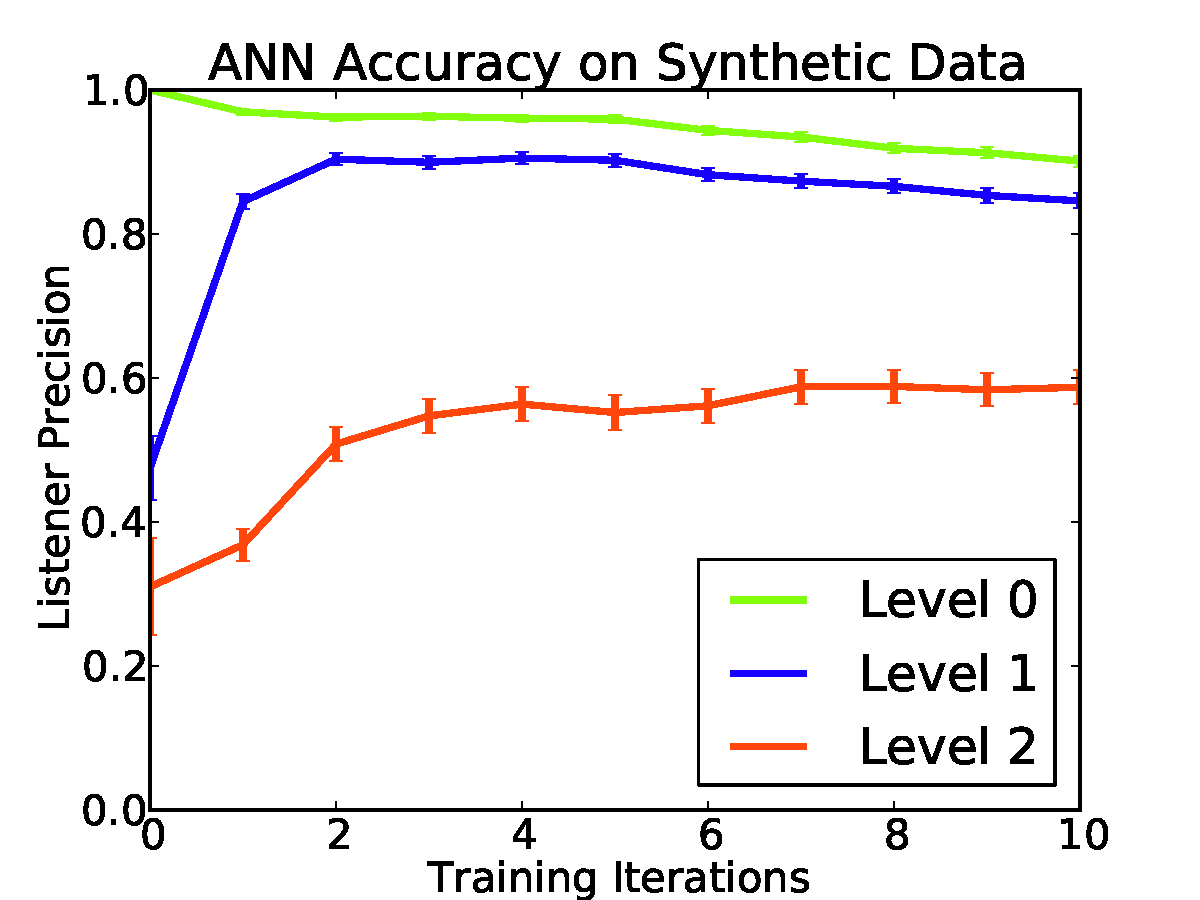
\includegraphics[width=\columnwidth]{fig/synthetic.pdf}
%    \caption {Listener accuracy on synthetic problems by number of training iterations, for a model with 50 hidden nodes.}
%    \label{fig:synthetic}
%\end{figure}
%
%\begin{figure}
%  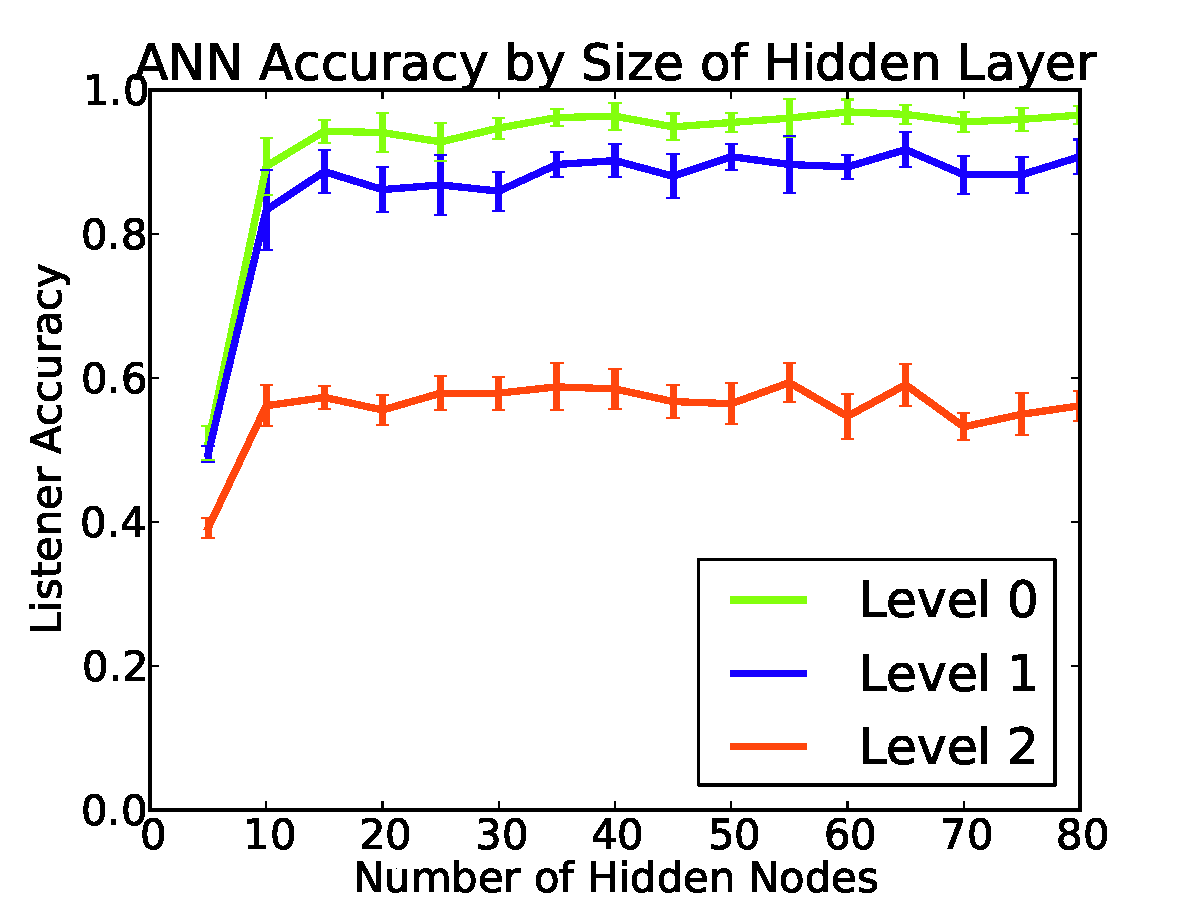
\includegraphics[width=\columnwidth]{fig/hiddenSynthetic.pdf}
%  \caption {Listener accuracy on synthetic problems while varying the size of the hidden layer.}
%  \label{fig:syntheticHidden}
%\end{figure}

\subsection{Discussion}

Model accuracy decreases as the problem level (complexity) increases.
The literal speaker performs perfectly on level~0 problems, as
expected. It is surprising that the trained models perform less than
perfectly on these easy problems. A listener trained \emph{only} on
level 0 problems achieves perfect accuracy on level~0 problems, so it
seems that training on the more difficult problems leads to some
degradation in performance on easy problems. The trained listeners
perform well, with 91\% accuracy on level~0, 85\% on level~1 problems,
and 59\% on level~2 problems.
Figure~\ref{fig:syntheticHidden} shows that the size of the hidden layer 
has some effect on model performance, but that after a certain threshold 
the performance stabilizes.

We also evaluated IBR listener models for a variety of recursion 
depths (Figure~\ref{fig:syntheticIBR}). All have perfect accuracy on
the level 0 problems (barely visible along the top of the plot), with
rapidly increasing accuracy on the level 1 and 2 problems. The
accuracies shown here are using the probabilities of each target given
a message \citep{Frank:Goodman:2012,Bergen:Goodman:Levy:2012}. If we
instead always choose the target with the highest probability given a
message \citep{Franke09DISS,Jaeger:2007,Jaeger:2011}, the IBR model
solves the problems exactly after one and two levels, respectively.

\begin{figure}[ht]
  \centering
  \subfigure[Varying the number of training iterations, with 50 hidden nodes.]{
    \parbox[c]{\columnwidth}{
      \centering
      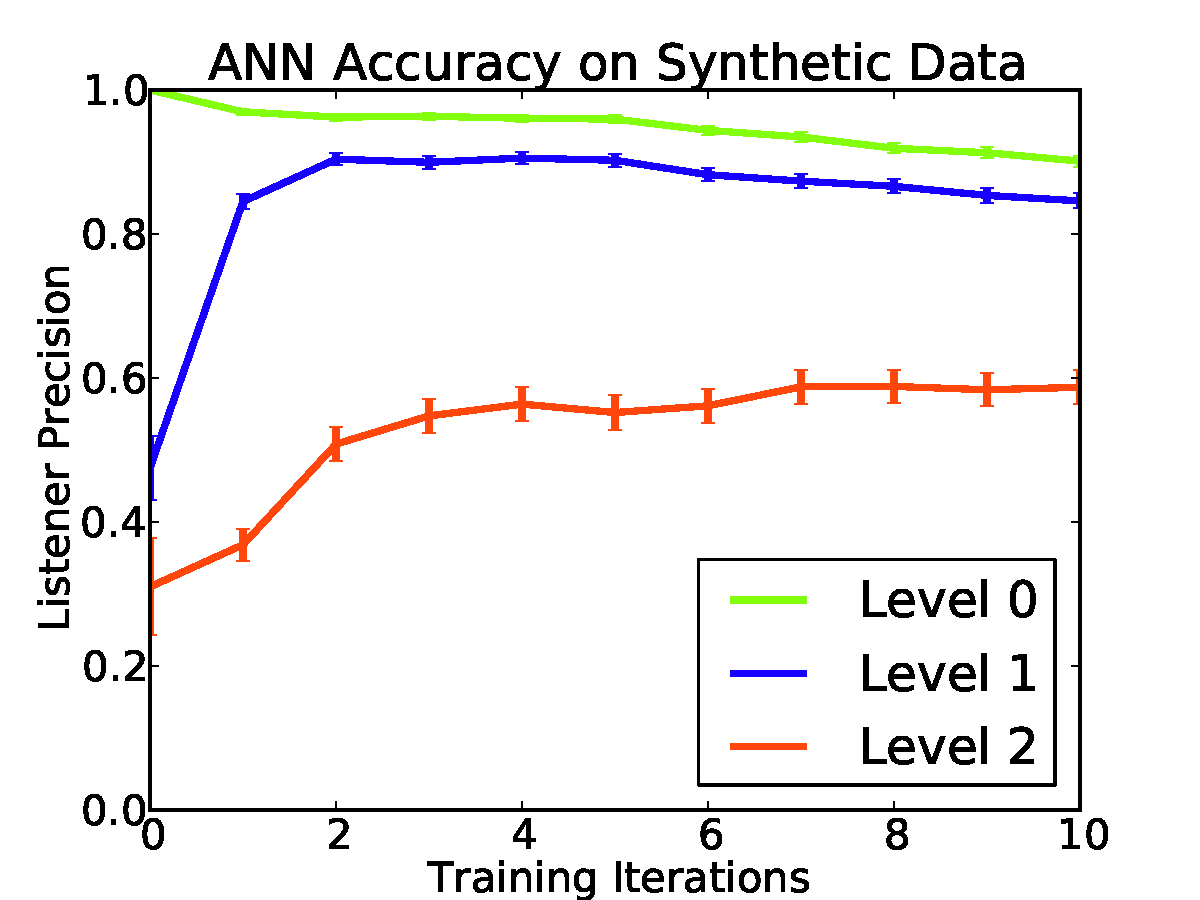
\includegraphics[width=0.8\columnwidth]{fig/synthetic.pdf}
    }
    \label{fig:synthetic}
  }

  \vspace{-2mm}

  \subfigure[Varying the number of hidden nodes, for 10 training iterations.]{    
    \parbox[c]{\columnwidth}{
      \centering
      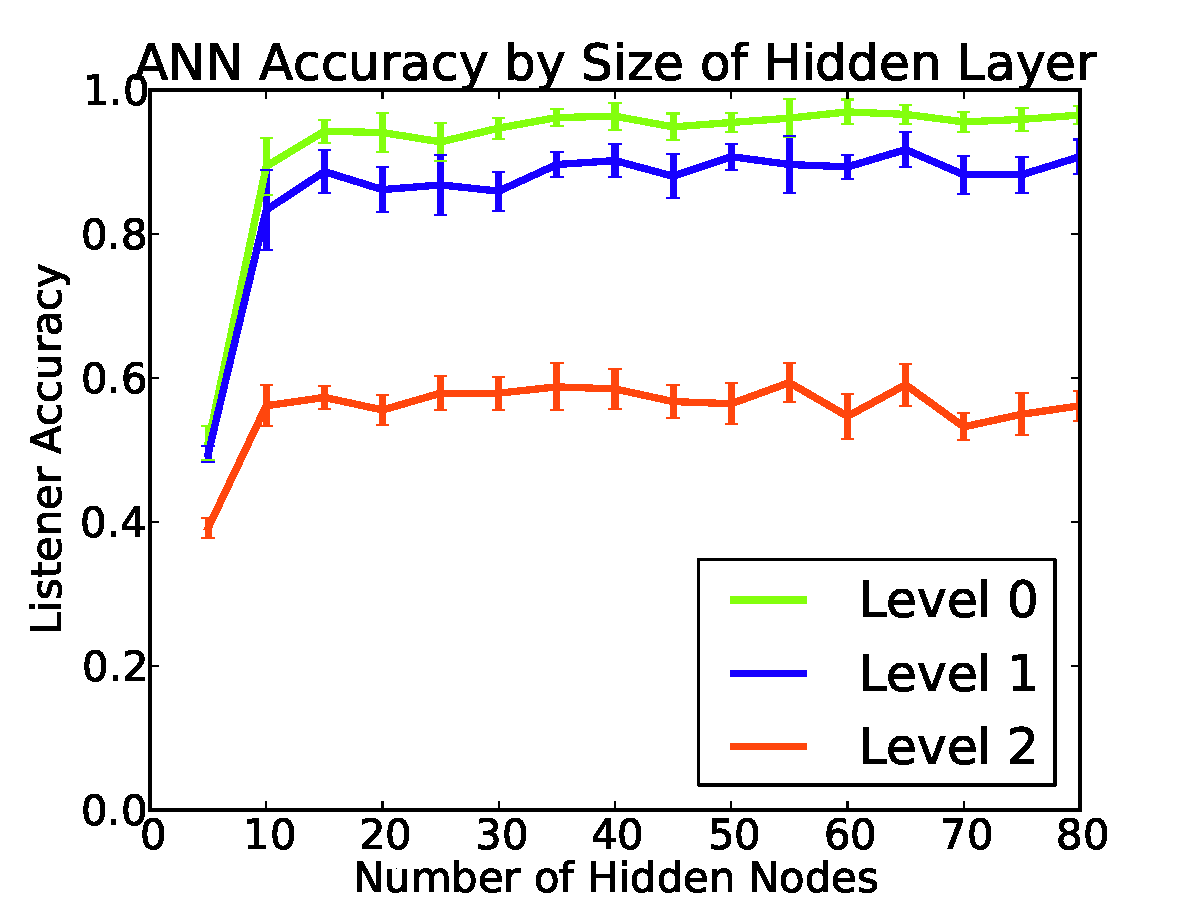
\includegraphics[width=0.8\columnwidth]{fig/hiddenSynthetic.pdf}
    }
    \label{fig:syntheticHidden}
  }
  \vspace{-4mm}
  \caption{ANN Listener accuracy on synthetic data.}
\end{figure}

\begin{figure}[ht]
  \centering
  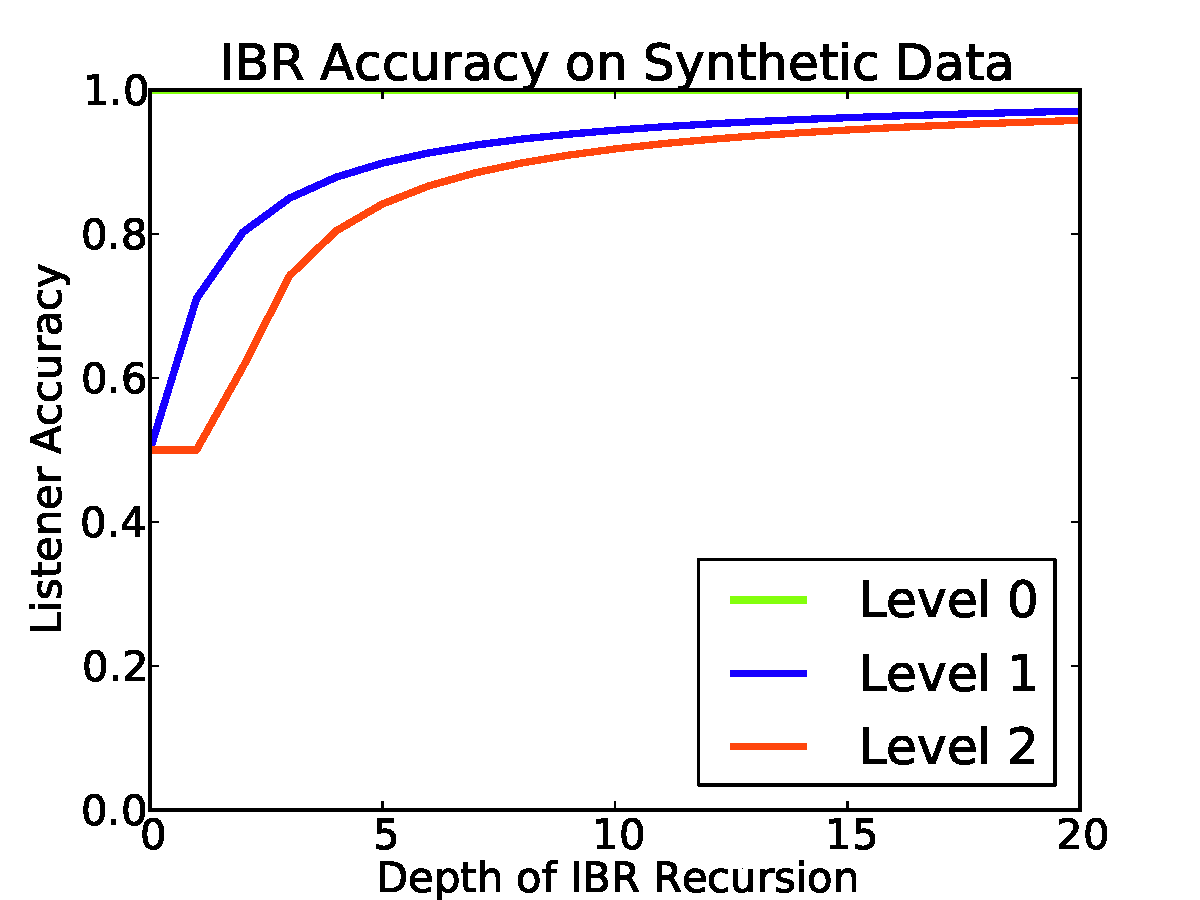
\includegraphics[width=0.8\columnwidth]{fig/IBRsynthetic.pdf}
  \vspace{-4mm}
  \caption{IBR listener accuracy on synthetic problems.}
  \label{fig:syntheticIBR}
\end{figure}
